\documentclass[../main.tex]{subfiles}

\begin{document}

\chapter{Об’єктно-орієнтоване проектування ІС}

Якщо аналіз об’єкта проектування – це розробка відповідної логічної моделі, яка описує усі можливі та прийнятні варіанти розв’язання задач, які вказують, що повинна робити система, то проектування – це вироблення рішення відповідно до моделі аналізу, яке оптимізує набір критеріїв проектування, які  показують, як ця поведінка (робота) системи може бути реалізована \cite{diploma_guidelines}.
Оскільки, у даній роботі застосовується об’єктно-орієнтована технологія проектування, то проектна частина повинна складатися із таких етапів:

\begin{enumerate}
	\item Архітектурне проектування – описує логічну структуру інформаційної системи (програмні класи, підсистеми,  пакети) та їх зв’язки.
	\item Детальне проектування – описує структури даних та алгоритми всередині окремих класів. 
\end{enumerate}

\section{Архітектурне проектування}
Формування архітектури – перший і основний крок у розв’язанні завдання проектування, що закладає фундамент уявлення програмної системи, здатної виконувати весь спектр детальних вимог. \cite{diploma_guidelines2}

Створення архітектури – це проектування на найвищому рівні (логічна архітектура). Логічна архітектура описує систему в термінах її принципової організації у вигляді пакетів, програмних класів і підсистем. Вона називається логічною, оскільки не визначає способи розгортання цих елементів у різних операційних системах або на фізичних комп’ютерах в мережі (це відноситься до архітектури розгортання) \cite{diploma_guidelines}.

Одним з найважливіших етапів архітектурного проектування є побудова діаграми пакетів. 

Діаграма пакетів є діаграмою, яка містить пакети класів і залежності між ними. Вона описує архітектурну основу системи і допомагає в управлінні масштабами і складністю системи. Діаграма пакетів для інформаційної системи зображена на рис. \ref{diagram:3.1}
\vspace{\baselineskip}

%TODO: change diagram after refactoring

\begin{figure}[H]
	\centering
	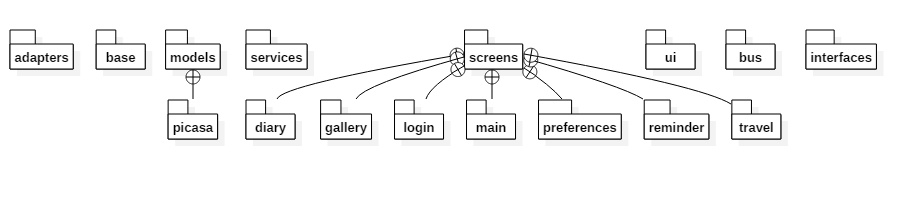
\includegraphics[width=1\textwidth]{diagram_packages}
	\caption{Діаграма пакетів інформаційної системи}
	\label{diagram:3.1}
\end{figure}

Ще одним будівельним блоком для створення архітектури об'єктно-орієнтованої системи вважається компонент. \cite{diploma_guidelines}

Діаграма компонентів показує розбиття програмної системи на структурні компоненти та залежності між компонентами. В якості фізичних компонентів можуть бути файли, бібліотеки, модулі, виконувані файли, пакети і т.п. У багатьох середовищах розробки модуль або компонент відповідає файлу. Стрілки, що з'єднують модулі, показують відносини взаємозалежності аналогічні тим, які мають місце при компіляції вихідних текстів програм. Основними графічними елементами діаграми компонентів є компоненти, інтерфейси і залежності між ними. Діаграму компонентів для інформаційної системи зображено на рис. \ref{diagram:3.2}

\begin{figure}[H]
	\centering
	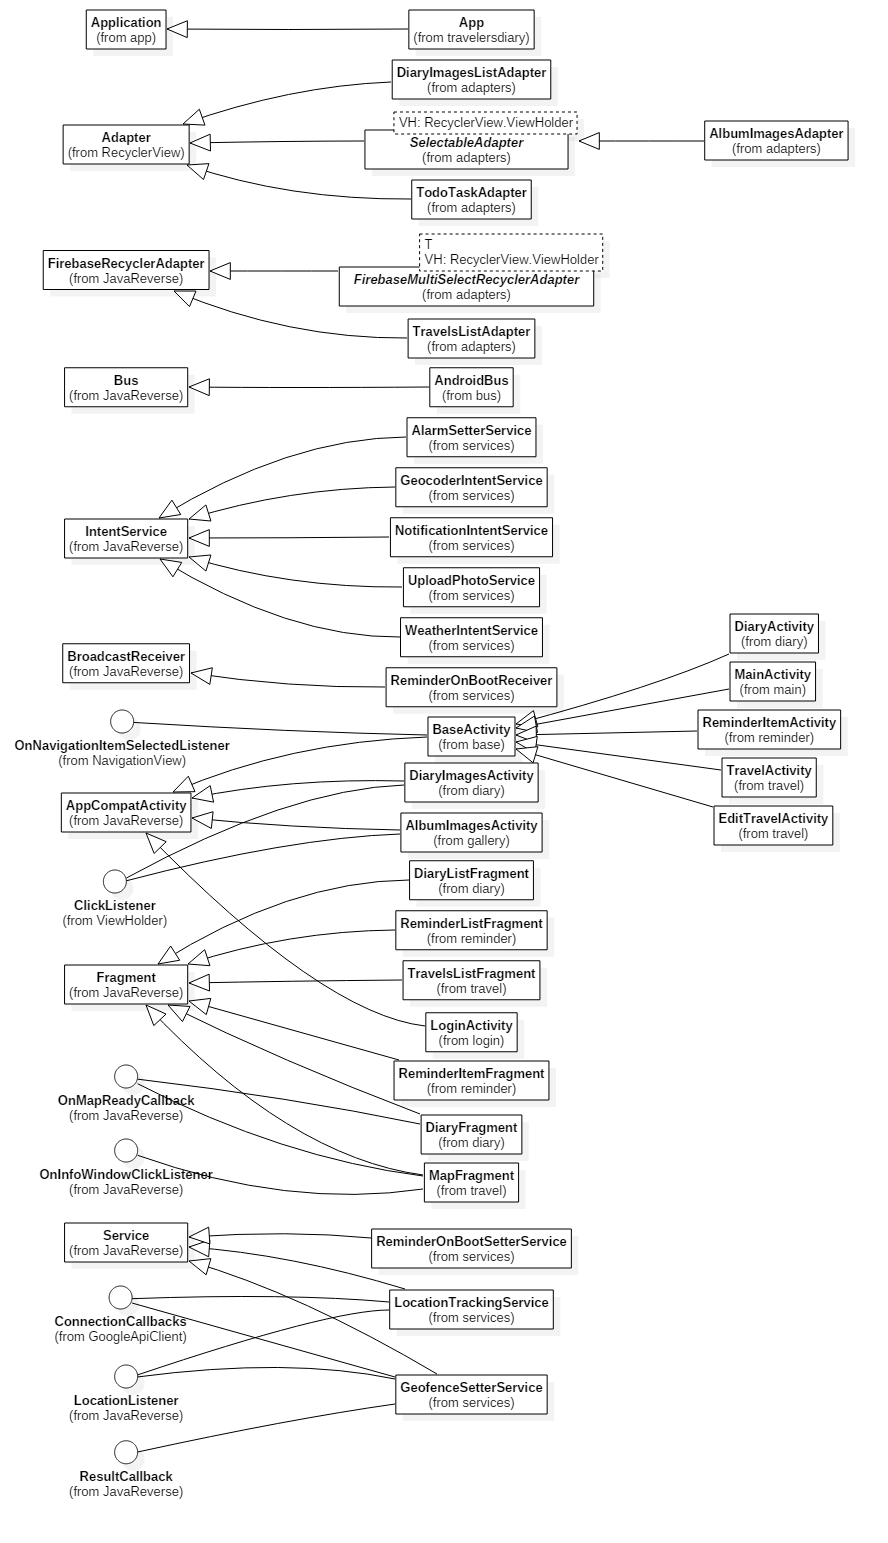
\includegraphics[height=0.8\textheight]{diagram_hierarchy}
	\caption{Діаграма компонентів Android додатку}
	\label{diagram:3.2}
\end{figure}

\section{Детальне проектування}

Детальне проектування – описує структури даних та алгоритми всередині окремих класів [10]. 

У програмуванні структури даних ‒ це способи організації даних в комп’ютерах. Часто разом зі структурою даних пов’язується і специфічний перелік операцій, які можуть бути виконаними над даними.
Правильний підбір структур даних є надзвичайно важливим для ефективного функціонування відповідних алгоритмів їх обробки. Добре побудовані структури даних дозволяють оптимізувати використання машинного часу та пам’ятті комп’ютера для виконання найбільш критичних операцій.

Логічна будова інформаційної системи (див. рис. \ref{diagram:3.3}) побудована  за допомогою UML-діаграми класів, яка служить для представлення статичної структури моделі системи в термінології класів об’єктно-орієнтованого програмування.

\begin{figure}[H]
	\centering
	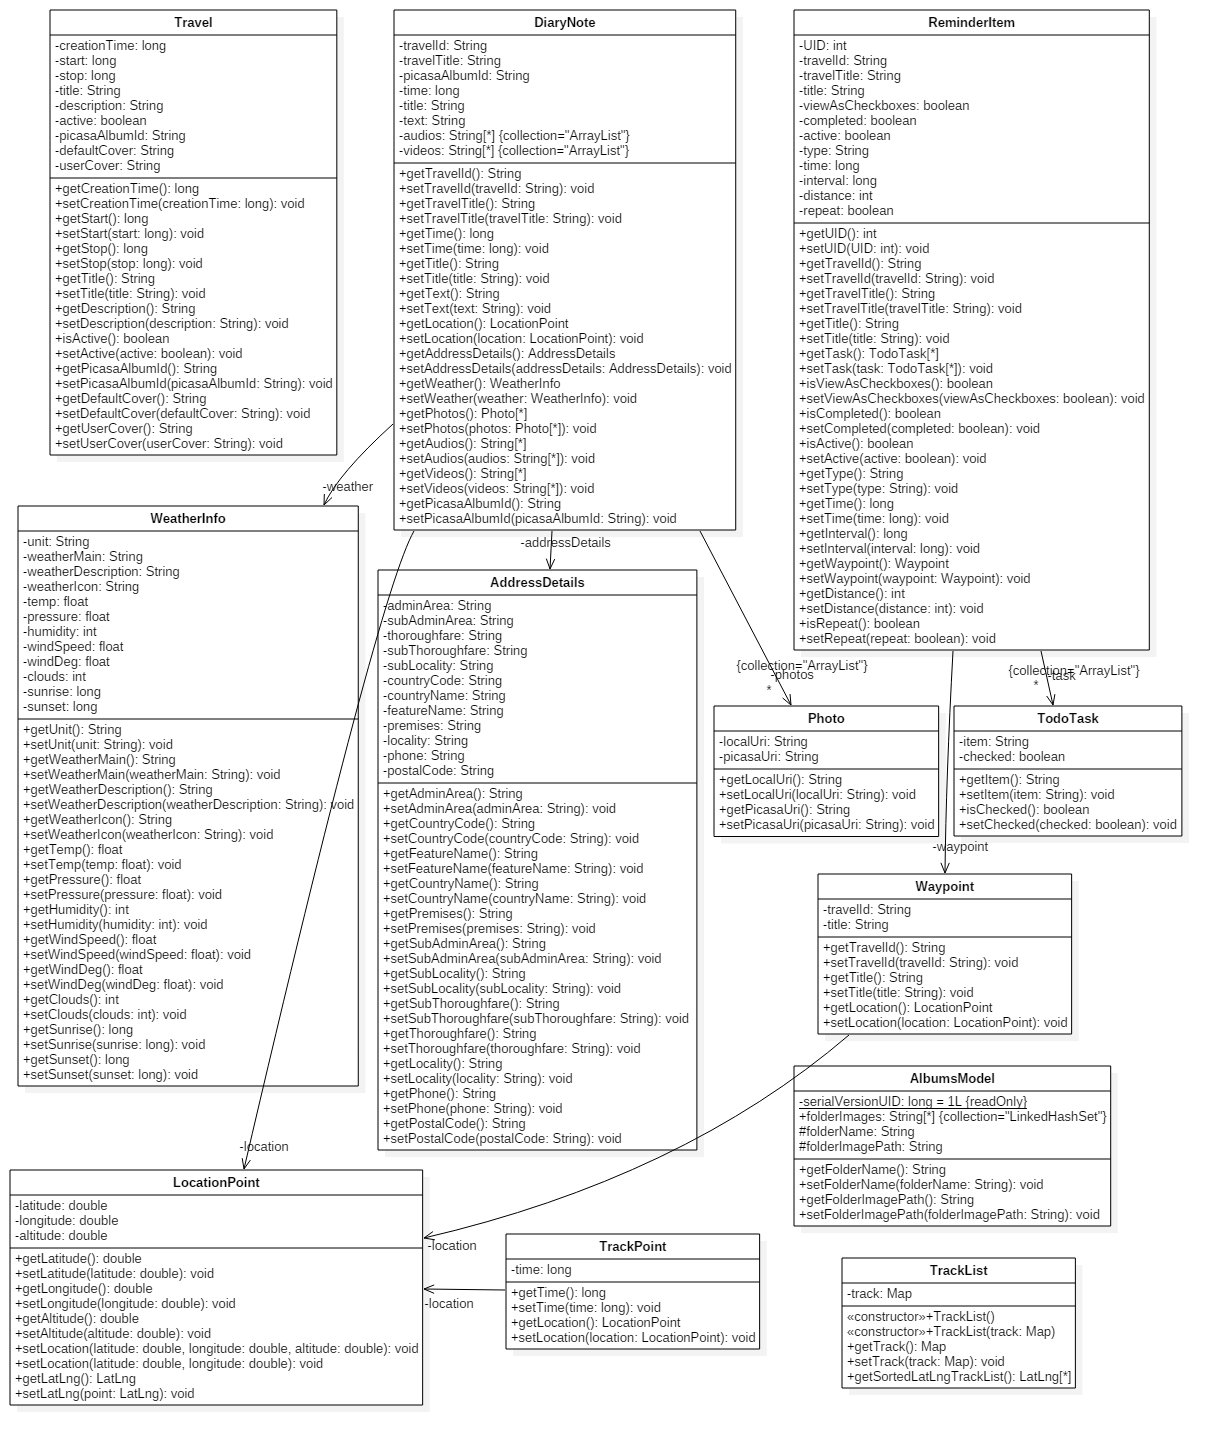
\includegraphics[height=0.8\textheight]{diagram_models}
	\caption{Діаграма моделей інформаційної системи}
	\label{diagram:3.3}
\end{figure}

%TODO: add models description


\section{Розгортання програмної системи на апаратних засобах}

Для функціонування додатку необхідна операційна система Android версії 4.2 (API 16) і вище.

%TODO: add something here


%TODO: Висновки до розділу (не більш 1-2 сторінки). Розмір одного висновку приблизно – один абзац (5-7 рядків). Висновки цього розділу є важливою і значущою частиною роботи.

\end{document}